\documentclass[norsk]{article}
\usepackage[utf8]{inputenc}
\usepackage[norsk]{babel}
\usepackage{hyperref}
\usepackage{listings}
\usepackage{titling}
\usepackage{tikz}
\usepackage{float}
\usepackage{cleveref}

\hypersetup{colorlinks=true,urlcolor=blue}

\setlength{\droptitle}{-10em}   % This is your set screw
%\posttitle{\par\end{center}\vspace{-10ex}}

\renewcommand{\familydefault}{\sfdefault}

\oddsidemargin=31pt
\topmargin=20pt
\headheight=12pt
\headsep=25pt
\textheight=592pt
\textwidth=430pt
\marginparsep=10pt
\marginparwidth=35pt
\footskip=30pt

\marginparpush=7pt
\hoffset=0pt
\voffset=0pt


\title{Oblig 2 -- INF1060 -- høst 2017}
\date{}

\begin{document}

\maketitle
\noindent I denne oppgaven skal du bruke det du har lært til nå og gjort i oblig 1, og kombinere det med filbehandling og kall til Linux-systembiblioteket. Vi skal med andre ord jobbe med filer, structer, strenger, pekere og systemkall.

Oppgavene skal løses selvstendig, se ellers \href{http://www.uio.no/studier/admin/obligatoriske-aktiviteter/mn-ifi-oblig.html}{Obligreglementet}. Du vil finne nyttige ukesoppgaver med tilhørende forklaringer av viktige begreper på  \href{http://folk.uio.no/hpkragse/INF1060/index.html}{gruppelærersiden}, og som i de fleste fag er \href{http://www.uio.no/studier/emner/matnat/ifi/INF1060/h17}{semestersiden} stedet for forelesningsfoiler og annen informasjon du kanskje er på utkikk etter.

Dersom du har spørsmål underveis kan du oppsøke en orakeltime eller stille spørsmål på \href{http://www.piazza.com/class}{Piazza}. Det vil (selvfølgelig) være mye relevant informasjon i plenumstime.

\textbf{Husk å lese hele oppgaveteksten}, så du vet hvor mye arbeid du har igjen totalt sett. \textit{Du vil til slutt i dokumentet finne en liste som viser hva du bør prioritere når du jobber med oppgaven.}

Oppgavene blir testet på Linux på Ifi sine maskiner eller tilsvarende.

\textbf{Innlevering i Devilry innen 3.\ oktober 23:59}

\section*{Oppgaven}

Vi tenker oss et scenario der IFI-Drift ønsker et \textquotedblright~bedre\textquotedblright~system for å administrere ruterne de har i drift ved Ole Johan Dahls og Kristen Nygaards hus. Drift vil ha et program som skal bli brukt til å lagre og behandle grunnleggende informasjon om ruterne. Programmet skal kjøres fra en terminal på et Linux-system, under kjøring skal bruker kunne se på og endre data om ruterne, og mellom kjøringer skal dataene være lagret i en fil.

Programmet skal kompileres med make (\textbf{dere må altså lage en makefile}), og startes med et filnavn som eneste argument. Filnavnet skal da være navnet på en fil som inneholder data om rutere som kan leses og behandles av programmet. For eksempel kan man starte på denne måten:

\begin{verbatim}
    $> ./ruterdrift 1router.dat
\end{verbatim}

Du finner flere data-filer du kan teste programmet ditt med i \href{http://github.uio.no/INF1060/Oblig2}{Oblig2-repositoriet på github}

\subsection*{Filstruktur}
Filen inneholder all data som programmet trenger. Filen har ikke (eksklusivt) tekst-data og kan dermed \textit{ikke} inspiseres i standard teksteditorer som Atom/Notepad etc. Dette er ment for å gjøre det enklere å skrive kode for å lese inn talldata, da man ikke trenger å tenke på å gjøre om mellom tall i tekstform og faktiske tall i minnet.

Det første som ligger i filen er en \texttt{int}, et 4-byte tall, som forteller oss hvor mange rutere filen har informasjon om. Informasjon om hver ruter er avgrenset med linjeskift, altså er hver ruter en \textquotedblleft~linje \textquotedblright~med informasjon. En gyldig fil uten ruterdata inneholder derfor én linje med kun tallet 0. \textit{Det er viktig å merke seg at denne første linjen er en 4-byte int-verdi, og ikke et tall på leselig form}! Resten av linjene er maksimalt 256 bytes lange (denne restriksjonen skal opprettholdes når man skriver ny data til fil). Se slutten av dokumentet for hint angående håndtering av binærdata i filer.

\clearpage

\noindent Hver av de etterfølgende linjene i filen representerer én ruter på følgende form:

\begin{itemize}
    \item Ruter-ID (unik) -- \texttt{unsigned char}
    \item FLAGG -- \texttt{unsigned char}
    \item Lengde på produsent/modell-strengen -- \texttt{unsigned char}
    \item Produsent/modell -- \texttt{char[]} (maks lengde 253)
\end{itemize}

Hver linje i filen inneholder altså 3 bytes med info om ruteren, etterfulgt av produsent/modell. Innad i programmet kan dere bruke en \texttt{struct} med disse akkurat lik definisjon som over.

\noindent Merk at siste felt i structen er et char-array, og dette kan åpne opp for noen spennende muligheter for spesielt interesserte, se seksjonen \textquotedblleft~Flexible array member\textquotedblright.

I hver struct skal det være en unsigned char, som i listen over heter FLAGG, og den skal representere diverse egenskaper en ruter kan ha. Flagg-feltet er forsøkt forklart i \cref{tab:flagg} og \cref{fig:flagg}.

\begin{table}[H]
    \centering
    \begin{tabular}{c|l|l|c}
        Bit-posisjon & Egenskap & Forklaring & Bokstav (for \cref{fig:flagg})\\
        \hline
        0 & Aktiv & Er ruteren i bruk? & A \\
        1 & Trådløs & Er ruteren trådløs? & B \\
        2 & 5GHz & Støtter ruteren 5GHz? & C \\
        3 & \textit{Ubrukt} & Ikke i bruk & D \\
        4:7 & Endringssnummer & Se lenger nede for info & \\
    \end{tabular}
    \caption{De ulike bitsene i flagg-feltet}\label{tab:flagg}
    \vspace{1cm}
\end{table}

\textbf{Obs:} merk at flagg-feltet potensielt kan ha verdien $'\backslash n'$, som vil terminere et kall på \texttt{fgets()} dersom dette er brukt for å lese linjen fra filen.

\begin{figure}[H]
    \centering
    \begin{tikzpicture}
        \draw (0,0) rectangle (4,1) node[pos=.5] {Endringsnummer};
        \draw (4,0) node[above=3em] {4};
        \draw (4,0) rectangle (5,1) node[pos=.5] {D};
        \draw (5,0) node[above=3em] {3};
        \draw (5,0) rectangle (6,1) node[pos=.5] {C};
        \draw (6,0) node[above=3em] {2};
        \draw (6,0) rectangle (7,1) node[pos=.5] {B};
        \draw (7,0) node[above=3em] {1};
        \draw (7,0) rectangle (8,1) node[pos=.5] {A};
        \draw (8,0) node[above=3em] {0};
    \end{tikzpicture}
    \caption{Flagg-feltet}\label{fig:flagg}
    \vspace{1cm}
\end{figure}

\section*{Spesifikasjoner}

Her er litt mer spesifikk informasjon om hva en bruker skal kunne bruke programmet til, og hvordan programmet skal fungere. Grovt sett vil programmet være delt i tre:

\begin{enumerate}
    \item Les inn filen og opprett de datastrukturer du trenger.
    \item Ordrestyrt program (\textquotedblright~ordreløkke\textquotedblright) der brukeren gir kommando og programmet utfører brukerens ønsker.
    \item Avslutning og skriving til fil.
\end{enumerate}

\subsection*{Innlesing og datastrukturer}
Dette skal skje med en gang programmet starter. Filen som er gitt som argument til programmet skal leses inn og dataen skal lagres i minne. For hver linje i filen skal det allokeres plass til en struct (med \texttt{malloc}), og structen skal fylles med data fra linjen. En peker til structen skal lagres i et globalt, statisk allokert (ikke \texttt{malloc}) array som vi skal bruke som et map. Mappet skal bruke ruter-ID som nøkkel og peker til ruter-strukten for den IDen som verdi, det hele er forsøkt illustrert i \cref{fig:map}. Når alle linjene har blitt lest inn, fått sin egen struct og sin egen entry i det globale mappet går programemt videre til ordreløkken.


\begin{figure}
    \centering
    \begin{tikzpicture}[scale=0.9]
    
        \draw (0,0) rectangle (3,6);
        \draw (0,1) -- (3,1);
        \draw (0,2) -- (3,2);
        \draw (0,3) -- (3,3);
        \draw (0,4) -- (3,4);
        \draw (0,5) -- (3,5);
        \draw[dashed] (0,0) -- (0,-1);
        \draw[dashed] (3,0) -- (3,-1);
        \node at (0.5,6.5) {Map};
        \node at (1.1,3.5) {struct-peker};
        \node at (-1,3.5) {Indeks 2};
        \draw[-{>[scale=3.0]}] (2.5,3.5) -- (6,4);
    
        \draw (6,0) rectangle (9,4);
        \draw (6,1) -- (9,1);
        \draw (6,2) -- (9,2);
        \draw (6,3) -- (9,3);
        \node at (7,4.5) {Ruter-struct};
        \node at (7,3.5) {Ruter-ID 2};
        
        
    \end{tikzpicture}
    \caption{Globalt map for rutere}\label{fig:map}
\end{figure}

\subsection*{Ordreløkke}
Programmet skal kjøre i loop, og gi brukeren mulighet til å gjøre følgende operasjoner:

\begin{itemize}
    \item Printe info om ruter gitt en ID
    \item Endre flagg for en ID
    \item Endre produsent/modell for en ID
    \item Legge inn en ny ruter (bruker putter inn ID og annen data)
    \item Slette en ruter fra databasen
    \item Avslutte programmet
\end{itemize}

Det er opp til deg hvordan du velger å løse ordreløkke-biten av oppgaven. Du kan selv velge om du vil ha en kommando-basert interaksjon med brukeren (et shell), eller om du vil printe en meny og la brukeren velge menyvalg, f.eks.\  ved tall. Uansett hvordan du velger å løse oppgaven bør det være intuitivt og enkelt å bruke programmet.

Det bør være intuitivt hvordan dataene i filen kan endres, for eksempel endring av navn og sletting av rutere. Det eneste som kanskje ikke er helt logisk er endringsnummeret i flagg-charen. Dette er et 4-bits tall som skal økes med $1$ hver gang det gjøres en endring på ruteren. Dersom tallet er 15 (binær $1111$) og brukeren forsøker å gjøre en endring, skal programmet nekte å gjennomføre endringen.

\subsection*{Avlutning}
Når brukeren velger å avslutte programmet skal alle allokerte minneområder (allokert med \texttt{malloc}) frigis ved kall på \texttt{free}, data skal skrives til den samme filen som den ble lest fra (overskrive hele filen), og filen skal lukkes.

Ekstraoppgave: Sett opp en signal-handler som gjør at brukeren også kan trykke \texttt{Ctrl-C} for å terminere programmet, uten at dette fører til minnelekasjer eller tap av data.

\subsection*{Viktighet av de forskjellige funksjonalitetene}

Her er en liste over viktigheten av de forskjellige delene av oppgaven. Bruk listen som en guide for hva du bør jobbe med (og i hvilken rekkefølge). Dette er med tanke på hva som blir viktig mot hjemmeeksamen og hva som er det sentrale ved oppgaven. Dette vil bli brukt ved retting.

\begin{enumerate}
    \item Innlesing av data fra fil
    \item Oppretting av map-strukturen
    \item Riktig innsetting av data i mappet
    \item God bruk av minne (\texttt{malloc} og \texttt{free})
    \item Endring av FLAGG-charen i en ruter-struct.
    \item Skriving av data til fil
    \item Fungerende brukerinteraksjon (ordreløkken)
    \item De resterende funksjonene (oprette, slette) er omtrent like viktige
\end{enumerate}

Med andre ord: \textbf{sørg for at innlesing og opretting av datastrukturen fungerer først, så sørg for å skrive til fil riktig. Pass på minnebruk hele veien.} Først når dette fungerer bør du begynne å se på de andre funksjonene i programmet.

\section*{Flexible array member (ekstraoppgave)}

De som vil ha litt ekstra moro og læring kan lese seg opp om det som kalles \textquotedblright~flexible array member\textquotedblright~i en strukt i C. Kort fortalt går det ut på at man kan ha en array uten lengde som siste element i en struct, og så allokere plass til structen + så mange array elementer man trenger, og deretter bruke array-feltet i structen til å indeksere utover den oprinnelige størrelsen til structen. Resultatet av å bruke dette er at vi allokerer ikke mer plass enn vi trenger til hver struct, og vi slipper å allokere to ganger ved å bruke en peker til et nytt allokert område.

Dette er en helt frivillig del av oppgaven.

\section*{Levering}

\begin{enumerate}
    \item Lag en mappe med ditt brukernavn: \texttt{mkdir bnavn}
    \item Kopier alle filene som er en del av innleveringen inn i mappen:\\ \texttt{cp *.c bnavn/} (f.eks.)
    \item Komprimer og pakk inn mappen:\\ \texttt{tar -czvf bnavn.tgz bnavn/}
    \item Logg inn på \href{http://devilry.ifi.uio.no}{Devilry}
    \item Lever under INF1060 Oblig X
\end{enumerate}

\newpage

\section*{Relevante man-sider}

Disse man-sidene inneholder informasjon om funksjoner som kan være relevante for løsing av denne oppgaven. Merk at
flere av man-sidene inneholder informasjon om flere funksjoner på én side, som \texttt{malloc/calloc/realloc}.

\begin{itemize}
    \item \texttt{malloc/calloc/realloc}
    \item \texttt{fgetc}
    \item \texttt{fread/fwrite}
    \item \texttt{fopen/fclose}
    \item \texttt{scanf/fscaf}
    \item \texttt{strcpy}
    \item \texttt{memcpy}
    \item \texttt{memmove}
    \item \texttt{atoi}
    \item \texttt{strtol}
    \item \texttt{isspace/isdigit/alnum} m.fl.
    \item \texttt{strdup}
    \item \texttt{strlen}
    \item \texttt{printf/fprintf}
\end{itemize}

\clearpage

\section*{Andre hint}

Da ruterdataen ikke kan leses som vanlig tekst er det lurt å ha en annen måte å inspisere filen(e) på. Til dette finnes blant annet terminalverktøyet \texttt{xxd}. Dette viser filen som hexadesimale tall ved siden av en tekstlig representasjon. Man kan da for eksempel enkelt se at de første fire bytene inneholder tallverdien som sier hvor mange rutere det er i filen.

\begin{figure}[H]
    \centering
    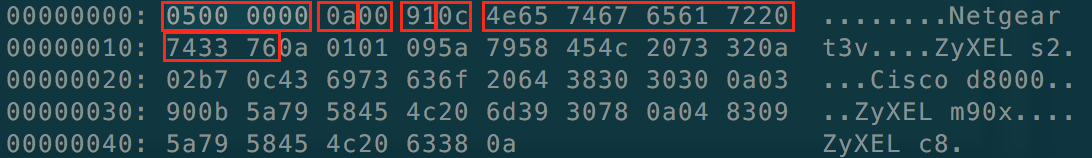
\includegraphics[width=\textwidth]{xxd_example.png}
    \caption{Eksempeloutput fra \texttt{xxd}}\label{fig:xxd}
    \vspace{1cm}
\end{figure}

\noindent \Cref{fig:xxd} viser \texttt{xxd}-output fra filen \texttt{5router.dat}. Hver hexadesimale siffer utgjør fire siffer i binært, altså trengs 2 hex-sifre for å representere én byte. De markerte rutene inneholder følgende data: 

\begin{itemize}
    \item \texttt{0500 0000} -- antall rutere i denne filen\footnotemark.
    \item \texttt{0a} -- karakteren \texttt{\textbackslash~n}, linjeskift. OBS:\@ denne kan forekomme ved uhell i flagg-feltet; det er ikke trygt å lese filen med \texttt{fgets}!
    \item \texttt{00} -- ruter-IDen for denne ruteren.
    \item \texttt{91} -- ruterens flagg. På binærform er dette \texttt{10010001}: Ifølge \cref{tab:flagg} betyr dette at ruteren er aktiv (bit på posisjon 0 er lik 1; vi sier at biten er \textit{satt}), og at den har blitt endret 9 ganger.
    \item \texttt{0c} -- lengden på strengen som inneholder produsent- og modellnavn. \texttt{0c} er 12 i desimal. Merk at linjeskiftet er medregnet.
    \item \texttt{4e65 7467 6561 7220 7433 76} -- strengen \textquotedblleft~Netgear t3v\textquotedblright.
\end{itemize}

\footnotetext{De spesielt interesserte kan lese om hvorfor den laveste byten er lagret først: \href{https://en.wikipedia.org/wiki/Endianness}{Wikipedia: Endianness}. Dette er ikke nødvendig kunnskap for å løse oppgaven.}

\end{document}

